\tikzset{every picture/.style={line width=0.75pt}} %set default line width to 0.75pt        

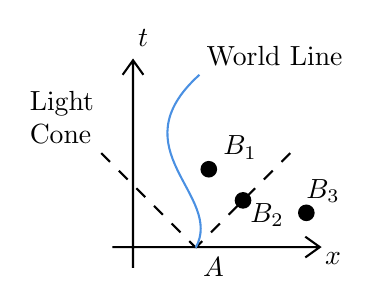
\begin{tikzpicture}[x=0.75pt,y=0.75pt,yscale=-1,xscale=1]
%uncomment if require: \path (0,300); %set diagram left start at 0, and has height of 300

%Shape: Axis 2D [id:dp6052588153202806] 
\draw  (214,173) -- (314,173)(224,83) -- (224,183) (307,168) -- (314,173) -- (307,178) (219,90) -- (224,83) -- (229,90)  ;
%Straight Lines [id:da10036025459043973] 
\draw  [dash pattern={on 4.5pt off 4.5pt}]  (299.78,127.72) -- (254.22,173.28) ;
%Straight Lines [id:da6125249800197986] 
\draw  [dash pattern={on 4.5pt off 4.5pt}]  (208.67,127.72) -- (254.22,173.28) ;
%Shape: Circle [id:dp934318391813717] 
\draw  [fill={rgb, 255:red, 0; green, 0; blue, 0 }  ,fill opacity=1 ] (257,135.5) .. controls (257,133.57) and (258.57,132) .. (260.5,132) .. controls (262.43,132) and (264,133.57) .. (264,135.5) .. controls (264,137.43) and (262.43,139) .. (260.5,139) .. controls (258.57,139) and (257,137.43) .. (257,135.5) -- cycle ;
%Shape: Circle [id:dp8271827138927054] 
\draw  [fill={rgb, 255:red, 0; green, 0; blue, 0 }  ,fill opacity=1 ] (273.5,150.5) .. controls (273.5,148.57) and (275.07,147) .. (277,147) .. controls (278.93,147) and (280.5,148.57) .. (280.5,150.5) .. controls (280.5,152.43) and (278.93,154) .. (277,154) .. controls (275.07,154) and (273.5,152.43) .. (273.5,150.5) -- cycle ;
%Shape: Circle [id:dp6545413454296474] 
\draw  [fill={rgb, 255:red, 0; green, 0; blue, 0 }  ,fill opacity=1 ] (304,156.5) .. controls (304,154.57) and (305.57,153) .. (307.5,153) .. controls (309.43,153) and (311,154.57) .. (311,156.5) .. controls (311,158.43) and (309.43,160) .. (307.5,160) .. controls (305.57,160) and (304,158.43) .. (304,156.5) -- cycle ;
%Curve Lines [id:da7989853479672057] 
\draw [color={rgb, 255:red, 74; green, 144; blue, 226 }  ,draw opacity=1 ]   (254.22,173.28) .. controls (268,148) and (216,126) .. (256,90) ;

% Text Node
\draw (225,78) node [anchor=south west] [inner sep=0.75pt]    {$t$};
% Text Node
\draw (315,174.4) node [anchor=north west][inner sep=0.75pt]    {$x$};
% Text Node
\draw (206.67,124.72) node [anchor=south east] [inner sep=0.75pt]   [align=left] {Light \\Cone};
% Text Node
\draw (256.22,176.68) node [anchor=north west][inner sep=0.75pt]    {$A$};
% Text Node
\draw (266,132.1) node [anchor=south west] [inner sep=0.75pt]    {$B_{1}$};
% Text Node
\draw (279,150.4) node [anchor=north west][inner sep=0.75pt]    {$B_{2}$};
% Text Node
\draw (306,153.1) node [anchor=south west] [inner sep=0.75pt]    {$B_{3}$};
% Text Node
\draw (258,87) node [anchor=south west] [inner sep=0.75pt]   [align=left] {World Line};


\end{tikzpicture}
